\section{Introduction}
A main objective of structural software testing is to achieve full or at least high code coverage such as statement and branch coverage of the program under test. A passing test suite that achieves high code coverage not only indicates the thoroughness of the testing but also provides high confidence of the quality of the program under test. Dynamic Symbolic Execution(DSE)\cite{CadarGPDE06,GodefroidKS05,SenMA05} is a variation of symbolic execution, which systematically explores feasible paths of the program under test by running the program with different test inputs to achieve high structural coverage. It collects the symbolic constraints on inputs obtained from predicates in branch statements along the execution and rely on a constraint solver, Z3 for Pex\cite{TillmannH08} and STP\cite{stp} for KLEE\cite{klee}, to solve the constraints and generate new test input for exploring new path. Currently, DSE works well in generating inputs for methods or parameterized unit tests with parameters of primitive type. However, when applying in object-oriented code, DSE could not easily generate inputs to achieve high structural coverage due to their little support for method sequence generation and floating point arithmetic, huge search space of feasible paths caused by loops and dependence of external library. Tackling these problems require complex analysis of the program and algorithms to find out solutions from a large possible space. But human, especially developers who write the program, could figure out the solution in a short time if provided the branch and statement coverage information with the relevant issues. Exsiting tools, like Pex, could report every issue encountered during the exploration, but some of the issues are actually not the cause of the problem. This will usually result in a long list of unordered issues, which makes it time consuming and tedious for user to figure out which action should be taken for guiding the DSE tool to increase the coverage.
\\In this paper, we propose an approach, Covana, which analyses the information collected during the DSE exploration, filters out the unrelevant information and report the not covered branches with the classified issues. To better inform user the problem, we define the categories of the issues which prevent the DSE technique to generate corresponding inputs:
\begin{itemize}
	\item object creation problem due to the limitation of method sequence generation 
	\item external library dependence, like uninstrumented method invocations
	\item environment dependence, like file system, database and so on
	\item explosion of feasible paths caused by loops or multi-level factory method (may not be examined)
\end{itemize}
Provided with the coverage information and the reported issue when DSE technique fails to generate an input for a paticular path, our approach is capable of locating the issues for a specific not covered branch and filtering out the unrelevant ones. In this way, user could browse the issues ordered by the not covered issues and target the problems directly. 
\\Our approach is built upon Pex, an white box test input generation tool developed by Microsoft Research. In order to obtain the coverage information and the issues reported during execution, we developed a Pex extension that serves as an observer to the different events occuring along the execution, collects the information of branch coverage and reported issues and save them into binary files. Given the information in files, we developed a tool that analyses these kinds of information, classifies the issues into the defined categories and attach the related issues to the not covered branches. 
\\Our detailed approach is:
\begin{enumerate}
\item Collects the branch coverage and find out the not covered branches. If the target statement of the not covered branch is covered, we simply filter out these not covered branches as it is useless for achieving higher coverage.
\item For the not covered branch which involves non-primitive object fields, we will search the reported issues to see whether there is an object creation issue for these fields. If found, we will consider this object creation issue is the cause which disallows Pex to cover the specific branch and report them with the not covered branch. 
\item For the uninstrumented method, we will make the method's return value as a symbolic and keep track of it. If there are not coverd branches whose constraints involve the symbolic we tracked, we will report it as the issue of external library dependence. Otherwise we will ignore it and discard the related information.
\item When DSE tool, like pex, fails to deal with the environment dependency or create an instance for some class which implements a specific interface, our tool will suggest user to use mock objects for solving these kind of problems.
\item When there is a explosion of feasible paths caused by loops, we will suggest ? (needs more experiments)
\end{enumerate}

 

%
%
%The objective of our approach is that if provided all the coverage information, like pex, developers need several changes and rerun the tool several times to make the branch covered, then adopting our approach could make the developers do it in fewer times or only one time.
%
%Here is my initial idea:
%
%1. Suggest the object based on the analysis of creation dependency.
%
%\begin{scriptsize}
%class Parent\{                                            	
%private Child child;                                      
%
%public CreateChild()\{                              
%	child = new Child();                                               
%\}
%
%public SetChildValue(int value)\{                              
%	child.value = value;                                              
%\}
%
%\}
%
%\end{scriptsize} 
%
%For this code snippet, we could see that the creation and modification of child object totally depends on its parent. Thus, if encountering some constraints involving child object's value, we should suggest the object creation of the parent but not the child. If the parent class provides constructor injection or setter injection for child object, then we should suggest improve the creation of the child object. This scenario also could be seen when constructor of child object is not visible.
%
%Solving this analysis problem could be a subtask.
%
%2. When applying pex in NHibernate, I found that when pex suggest creating an object with multiple fields, it will list all the fields in that class. But actually most of the fields are not relevant to the uncovered branch and could be filtered out. We could isolate these unrelevant fields and just list the fields involved in the constraints of the uncovered branch.
%
%3. When applying pex in NHibernate, I found that inside a method under test, there are several other method invocations, which increases the search space a lot for pex. However, some of the methods are not from the object under test and pex still tries to cover all the branches inside such methods. 
%
%Supposed we have a class parent with an uncovered branch which requires the evaluation of the child's method, to satisfy this constraint we only need to make the child's method return true.
%\begin{center}
%	\includegraphics[scale=0.42,keepaspectratio]{code1.eps}
%\end{center}
%
%\begin{center}
%	\includegraphics[scale=0.42,keepaspectratio]{code2.eps}
%\end{center}
%
%After digging into child's method, we could see that the method could have several paths to return true. I think here we do not need to explore every possible path of class child as our test target is parent, especially when child's methos is an uninstrumented method. We could just choose two values which statisfy the predict coverage of the child's method and the coverage of the parent would be fine. Currently pex will report every issue encountered during the exploration, no matter it is the class under test or not. In this simple example, pex is able to find out all the possible inputs for the child's method, CanUnderstand. However, in real application, like NHibernate or Quartz.NET, the call stack of external method invocation is deep and it is often involved many object creation issues, which make it impossible for pex to solve the constraint. Therefore, if we only satisfy the predict coverage of external method, like child's method, then we could reduce the pex's effort a lot.
%
%To provide more relevant information for developers, we could do static analysis of the external method. Taking the child's method, CanUnderstand, in figure 1 for example, to satisfy predict coverage, we only need to find out two path which make it return true and false respectively. Supposed pex is stuck for two constraints inside the external method, then we should rank the constraints and give the one which have fewer condition checks before it reaches the end of the method higher score. In the given example, supposed we want the method to return true and pex could not solve all the constraints that make it return true, we should rank the first constraint, value.Constains(``hi''), as there is no other condition check following it. 
%
%4. When pex is stuck for some condition check inside a private method, reporting the variable related to the constraints may not be so useful. See the example code from NHibernate below:
%
%\begin{verbatim}
%private bool IsEquals(ICollection x, ICollection y){
%	... 
%		if (x.Count != y.Count)
%					return false;
%	...
%}
%\end{verbatim}
%
%Given this code snippet, even we know x and y are related to the constraints, we have no way to figure it out what we could do to assist pex as we have no idea where and when the method is invoked during the execution. However, if we do keep a dataflow, then it could make things much easier. If we trace back the example code in NHibernate, we could find the method below:
%
%\begin{verbatim}
%public bool Equals(TypedValue x, TypedValue y)
%			{
%				if (y == null) return false;
%				if (!x.type.ReturnedClass.Equals(y.type.ReturnedClass))
%					return false;
%				return IsEquals(x.type, x.value as ICollection, 
%								y.value as ICollection);
%			}
%\end{verbatim}
%
%Here, ``Equals'' is the method under test and the actual arguments for the ``IsEquals'' method are just the ``value'' attribute of its own arguments x and y. By looking at this, we could know that to make that branch covered, we should add some method sequence to help pex assign the value to TypedValue.value. In this case, we could link the second method to the first one and report them together.
